\documentclass[11pt]{article}

\usepackage[hmargin=1in,vmargin=0.8in]{geometry}
\usepackage[T1]{fontenc}
\usepackage{lmodern}
\usepackage{microtype}
\usepackage{amsmath,amssymb,amsthm,mathtools}
\usepackage{mathrsfs}
\usepackage[dvipsnames]{xcolor}
\usepackage[most]{tcolorbox}
\usepackage{tikz}
\usetikzlibrary{decorations.markings,patterns}
\usepackage{enumitem}
\usepackage{tocloft}
\usepackage[hidelinks]{hyperref}

\definecolor{courseblue}{HTML}{1F4E79}
\definecolor{lightblue}{HTML}{EAF2F8}
\definecolor{lightgreen}{HTML}{EAF7EA}
\definecolor{lightpink}{HTML}{FCE8EF}
\definecolor{lightyellow}{HTML}{FFF8D6}
\definecolor{warningyellow}{HTML}{D6A000}
\definecolor{exercisebg}{HTML}{FDEAEA}
\definecolor{exerciseframe}{HTML}{B54040}
\definecolor{examplebg}{HTML}{F4FAFE}
\definecolor{exampleframe}{HTML}{85C1E9}
\definecolor{darkgray}{HTML}{333333}
\definecolor{lightorange}{HTML}{FDEBD8}
\definecolor{orangeframe}{HTML}{E08A3C}
\definecolor{remarkbg}{HTML}{F3EEFB}
\definecolor{remarkframe}{HTML}{9B7FC9}

\setlength{\parindent}{0pt}
\setlength{\parskip}{0.30em}
\setlist[itemize]{topsep=0.25em,itemsep=0.15em}
\renewcommand{\cftsecleader}{\cftdotfill{\cftdotsep}}
\renewcommand{\cftsubsecleader}{\cftdotfill{\cftdotsep}}

\theoremstyle{plain}
\newtheorem{theorem}{Theorem}[section]
\newtheorem{proposition}[theorem]{Proposition}
\newtheorem{lemma}[theorem]{Lemma}
\newtheorem{corollary}[theorem]{Corollary}
\theoremstyle{definition}
\newtheorem{definition}[theorem]{Definition}
\newtheorem{example}[theorem]{Example}
\newtheorem{exercise}[theorem]{Exercise}
\newtheoremstyle{boldremark}
  {3pt}{3pt}{\normalfont}{}{\bfseries}{.}{.5em}
  {\thmname{#1}\thmnumber{ #2}\thmnote{ (#3)}}
\theoremstyle{boldremark}
\newtheorem*{remark}{Remark}
\theoremstyle{remark}
\newtheorem*{fact}{Fact}
\newtheorem*{warning}{Warning}

\tcolorboxenvironment{definition}{
  enhanced,
  unbreakable,
  colback=lightgreen,
  colframe=ForestGreen,
  boxrule=0.7pt,
  arc=2pt,
  left=6pt,
  right=6pt,
  top=5pt,
  bottom=5pt
}

\tcolorboxenvironment{remark}{
  enhanced,
  colback=remarkbg,
  colframe=remarkframe,
  before upper={\setlength{\parskip}{0.5em}},
  boxrule=0.7pt,
  arc=2pt,
  left=6pt,
  right=6pt,
  top=5pt,
  bottom=5pt
}

\tcolorboxenvironment{warning}{
  enhanced,
  colback=lightyellow,
  colframe=warningyellow,
  boxrule=0.7pt,
  arc=2pt,
  left=6pt,
  right=6pt,
  top=5pt,
  bottom=5pt
}

\tcolorboxenvironment{exercise}{
  enhanced,
  colback=exercisebg,
  colframe=exerciseframe,
  boxrule=1pt,
  arc=2pt,
  left=6pt,
  right=6pt,
  top=5pt,
  bottom=5pt
}

\tcolorboxenvironment{example}{
  enhanced,
  colback=examplebg,
  colframe=exampleframe,
  boxrule=0.7pt,
  arc=2pt,
  left=6pt,
  right=6pt,
  top=5pt,
  bottom=5pt
}

\numberwithin{equation}{section}

\newcommand{\be}{\begin{eqnarray}}
\newcommand{\ee}{\end{eqnarray}}
\newcommand{\C}{\mathbb{C}}
\newcommand{\R}{\mathbb{R}}
\newcommand{\N}{\mathbb{N}}
\newcommand{\Z}{\mathbb{Z}}
\DeclareMathOperator{\Log}{Log}
\DeclareMathOperator{\Arg}{Arg}

\DeclareMathOperator{\Hol}{\mathcal{H}\mathrm{ol}}
\DeclareMathOperator{\Real}{Re}
\DeclareMathOperator{\Imag}{Im}
\newcommand{\A}{\mathcal{A}}
\newcommand{\CT}{\C[[T]]}
\newcommand{\CLT}{\C((T))}
\tcbset{breakable}
% Compact spacing around diagrams; keep the main text at 11pt.
\newenvironment{lecturefigure}
 {\par\addvspace{0.25em}\begingroup\setlength{\parskip}{0pt}\centering}
 {\par\endgroup\addvspace{0.25em}}
\begin{document}

\begin{center}
  \colorbox{lightblue}{%
    \begin{minipage}{0.94\textwidth}
      \vspace{0.55em}
      \begin{tabular*}{\textwidth}{@{\extracolsep{\fill}}lr}
        {\color{courseblue}\bfseries\LARGE Lecture 26} &
        {\color{courseblue}\bfseries\LARGE MATH 411}\\[0.35em]
        \textbf{Fall 2026} & \textbf{Date: Nov 18, 2026}\\
        & \textbf{Instructor: Manish Patnaik}
      \end{tabular*}
      \vspace{0.45em}
    \end{minipage}}
\end{center}

\setcounter{tocdepth}{1}
\tableofcontents
\vspace{0.45em}

% Sources: typed Lecture 25 from the argument principle to the end
% (handwritten Lecture 24, pages 2--6), followed by all new material in
% handwritten Lecture 25, Nov. 16, pages 1--4.
In Lecture~25 we studied improper integrals and the order of a zero or
pole. We now begin with the argument principle and use it to prove
Rouch\'e's theorem and the open mapping theorem. We then deduce the
maximum modulus principle and show that an injective holomorphic map
has a holomorphic inverse.

\section{The argument principle}
% Handwritten Lecture 24, pages 2--3.
Recall from Lecture~25 that, near a zero or pole $z_0$, a meromorphic
function has the form $f(z)=(z-z_0)^m g(z)$, where $g$ is holomorphic and
$g(z_0)\ne0$. Thus
\[
 \frac{f'(z)}{f(z)}=\frac{m}{z-z_0}+\frac{g'(z)}{g(z)},\qquad
 \operatorname{Res}_{z_0}\!\left(\frac{f'}{f}\right)
 =m=\operatorname{ord}_{z_0}(f).
\]
Combining this observation with the residue theorem gives the following.

\begin{theorem}\label{thm:log-derivative}
Let $U$ be open and $f$ meromorphic on $U$ with finitely many zeros and
poles $z_1,\dots,z_n$. Let $\gamma$ be a closed piecewise $C^1$ curve in
$U\setminus\{z_1,\dots,z_n\}$ that is null-homotopic in $U$. Then
\[
 \int_\gamma\frac{f'}{f}=2\pi i\sum_{j=1}^{n}w(\gamma,z_j)\,
 \operatorname{ord}_{z_j}(f).
\]
\end{theorem}
\begin{proof}
On $U\setminus\{z_1,\dots,z_n\}$, $f$ is holomorphic and nonvanishing, so
$f'/f$ is holomorphic there. At each $z_j$ it has residue
$\operatorname{ord}_{z_j}(f)$ by the computation above. Apply the residue
theorem to $f'/f$.
\end{proof}

\begin{example}
Let $f(z)=\dfrac{(z-1)^2}{(z+2)^3}$, with a zero of order $2$ at $1$ and a
pole of order $3$ at $-2$. For the circle $|z|=3$, both points are inside
and $\int f'/f=2\pi i(2-3)=-2\pi i$. For $|z|=\tfrac32$, only $1$ is inside
and $\int f'/f=4\pi i$. Directly,
$f'/f=\frac{2}{z-1}-\frac{3}{z+2}$.
\end{example}

Choosing $\gamma$ to be a circle gives the following.

\begin{corollary}[Argument principle]\label{cor:argument}
Let $C$ be a positively oriented circle bounding the open disc $D$, and
let $f$ be meromorphic on an open set $W\supseteq\overline D$, with finitely
many zeros and poles in $W$, none on $C$. Then
\[
 \boxed{\frac{1}{2\pi i}\int_C\frac{f'}{f}
 =\#\{\text{zeros of $f$ in $D$}\}-\#\{\text{poles of $f$ in $D$}\},}
\]
where zeros and poles are counted with multiplicity (that is, with their
orders).
\end{corollary}

\begin{remark}[Simple closed curves]
The circle $C$ may be replaced by any piecewise continuously differentiable,
positively oriented simple closed curve, with $D$ its interior. A closed
curve is \emph{simple} (non-self-intersecting) if it visits each point only once, except that its
starting and ending points coincide. It is \emph{positively oriented} if
the interior stays on your left as you travel along the curve.
\end{remark}

\begin{proof}[Proof of Corollary~\ref{cor:argument}]
Let $D=D(c,r)$. By compactness of $\overline D$ there is $\rho>r$ with
$D(c,\rho)\subseteq W$. Apply Theorem~\ref{thm:log-derivative} on the
convex, hence simply connected, set $U=D(c,\rho)$. It remains to note that
$w(C,\alpha)=1$ for $\alpha\in D$ (Cauchy's formula with $f=1$) and
$w(C,\alpha)=0$ for $|\alpha-c|>r$ (since $1/(z-\alpha)$ is holomorphic on
the disc $D(c,|\alpha-c|)$, which contains $C$).
\end{proof}

\begin{lecturefigure}
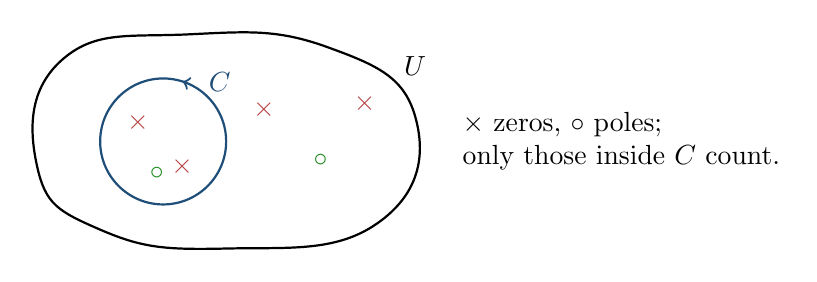
\begin{tikzpicture}[scale=0.8]
 \draw[thick] plot[smooth cycle,tension=0.8] coordinates
 {(-3,-0.4) (-2.6,1.3) (-0.6,1.7) (1.6,1.5) (3,0.4)
  (2.4,-1.3) (0,-1.7) (-2,-1.4)};
 \node at (3,1.2) {$U$};
 \draw[courseblue,thick,postaction={decorate},decoration={markings,
  mark=at position 0.2 with {\arrow{>}}}] (-1,0) circle(1);
 \node[courseblue] at (-0.1,0.95) {$C$};
 \node[exerciseframe] at (-1.4,0.3) {$\times$};
 \node[exerciseframe] at (-0.7,-0.4) {$\times$};
 \node[ForestGreen] at (-1.1,-0.5) {$\circ$};
 \node[exerciseframe] at (0.6,0.5) {$\times$};
 \node[ForestGreen] at (1.5,-0.3) {$\circ$};
 \node[exerciseframe] at (2.2,0.6) {$\times$};
 \node[right,align=left] at (3.6,0)
 {$\times$ zeros, $\circ$ poles;\\ only those inside $C$ count.};
\end{tikzpicture}
\end{lecturefigure}

\begin{remark}[Why ``argument'']
If $C$ is parametrized by $\gamma(t)$, $0\leq t\leq2\pi$, then
$\int_C f'/f=\int_0^{2\pi}\frac{(f\circ\gamma)'(t)}{f(\gamma(t))}\,dt
=\int_{f\circ C}\frac{dw}{w}$. So the left side of the argument principle
is $w(f\circ C,0)$: the number of times the image curve $f\circ C$ winds
around $0$, i.e.\ the total change in $\arg f(z)$ around $C$, divided by
$2\pi$.
\end{remark}

\begin{example}[Counting solutions from an ellipse]
Let $C$ be the positively oriented circle $|z|=2$, and set
$f(z)=z+1/z=(z^2+1)/z$. Inside $C$ there are two simple zeros at $\pm i$
and one simple pole at $0$. By the argument principle,
\[
 \int_C \frac{f'(z)}{f(z)}\,dz=2\pi i(2-1)=2\pi i.
\]
We can also see this from the image curve. Parametrize $C$ by
$C(t)=2e^{it}$ for $0\le t\le 2\pi$. Then
\[
 f(C(t))=2e^{it}+\tfrac12e^{-it}
        =\tfrac52\cos t+i\tfrac32\sin t.
\]
\begin{minipage}[c]{0.54\linewidth}
Writing $f(C(t))=x+iy$, we obtain the ellipse
\[
 \frac{x^2}{(5/2)^2}+\frac{y^2}{(3/2)^2}=1.
\]
The curve starts at $5/2$ and goes around the ellipse once
counterclockwise, so $w(f\circ C,0)=1$.
\end{minipage}\hfill
\begin{minipage}[c]{0.44\linewidth}
\centering
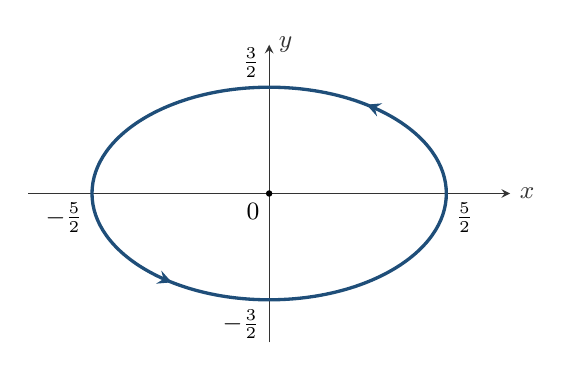
\begin{tikzpicture}[scale=0.9,>=stealth,font=\small]
 \draw[->,darkgray] (-3.4,0) -- (3.4,0) node[right] {$x$};
 \draw[->,darkgray] (0,-2.1) -- (0,2.1) node[right] {$y$};
 \draw[courseblue,very thick,postaction={decorate},decoration={markings,
   mark=at position 0.14 with {\arrow{stealth}},
   mark=at position 0.64 with {\arrow{stealth}}}]
   (2.5,0) arc[start angle=0,end angle=360,x radius=2.5,y radius=1.5];
 \node[below right] at (2.5,0) {$\tfrac52$};
 \node[below left] at (-2.5,0) {$-\tfrac52$};
 \node[above left] at (0,1.5) {$\tfrac32$};
 \node[below left] at (0,-1.5) {$-\tfrac32$};
 \fill (0,0) circle (1.3pt) node[below left] {$0$};
\end{tikzpicture}
\end{minipage}
\end{example}
 
\section{Rouch\'e's theorem}
% Handwritten Lecture 24, pages 3--5.
\begin{theorem}[Rouch\'e's theorem]\label{thm:rouche}
Let $f$ and $g$ be holomorphic on an open set containing a closed disc
$\overline D$ with boundary circle $C$, and suppose
\[
 |f(z)|>|g(z)|\qquad\text{for all }z\in C.
\]
Then $f$ and $f+g$ have the same number of zeros in $D$, counted with
multiplicity.
\end{theorem}

\begin{remark}
\leavevmode
\begin{enumerate}[leftmargin=*,nosep]
\item Note that the hypothesis forces $f\ne0$ on $C$. Think of $g$ as a
perturbation that is small on $C$: it does not change the number of zeros
inside.
\item The circle $C$ may be replaced by any piecewise continuously differentiable
simple closed curve. Let $D$ be its interior. If $f$ and $g$ are holomorphic
on a neighborhood of $\overline D$ and $|g(z)|<|f(z)|$ at every point of
$C$, then $f$ and $f+g$ have the same number of zeros in $D$, counted with
multiplicity. Either orientation of $C$ gives the same conclusion.
\end{enumerate}
\end{remark}

\begin{proof}[Proof of Theorem~\ref{thm:rouche}]
Let $D=D(c,r)$, and choose $\rho>r$ so that $f,g$ are holomorphic on
$D(c,\rho)$. Consider the ``deformations''
\[
 f_t=f+tg,\qquad t\in[0,1],
\]
so that $f_0=f$ and $f_1=f+g$. Let $n_t$ be the number of zeros of $f_t$ in
$D$. We want to show $n_0=n_1$.

\textbf{$f_t$ has no zeros on $C$.} If $f_t(z)=0$ with $z\in C$, then
$|f(z)|=t|g(z)|\leq|g(z)|$, contradicting $|g|<|f|$ on $C$. 

More
quantitatively, let us write $\mu:=\min_C(|f|-|g|).$ We note that by compactness, $$ \mu > 0. $$ Moreover, we also have on $C$: 
$$|f_t|\geq|f|-|g|\geq\mu.$$

\textbf{$n_t$ is given by the argument principle.} Since $f_t$ is not
identically zero on the connected set $D(c,\rho)$, the isolated-zero lemma
from Lecture~25 shows that it has finitely many zeros in the open disc $D(c,\rho')$ for any
$r<\rho'<\rho$. Since $f_t$ is holomorphic, it has no poles, so
Corollary~\ref{cor:argument} gives
\[
 n_t=\frac{1}{2\pi i}\int_C\frac{f_t'}{f_t}.
\]

\textbf{$t\mapsto n_t$ is continuous.} For $s,t\in[0,1]$, expanding
$(f'+sg')(f+tg)-(f'+tg')(f+sg)$ gives
\[
 \frac{f_s'}{f_s}-\frac{f_t'}{f_t}
 =\frac{f_s'f_t-f_t'f_s}{f_sf_t}
 =\frac{(t-s)\bigl(f'g-fg'\bigr)}{f_sf_t}.
\]
With $K=\max_C|f'g-fg'|$, the estimation lemma yields
\[
 |n_s-n_t|\leq\frac{1}{2\pi}\operatorname{Length}(C)\,
 \sup_{z\in C}\left|\frac{f_s'}{f_s}-\frac{f_t'}{f_t}\right|
 \leq\frac{1}{2\pi}\cdot2\pi r\cdot\frac{K}{\mu^2}\,|t-s|
 \longrightarrow0\quad(s\to t).
\]

\textbf{Conclusion.} A continuous integer-valued function on the connected
interval $[0,1]$ is constant. Hence $n_0=n_1$.
\end{proof}

\begin{example}
How many zeros does $P(z)=z^8-5z^3+z-2$ have in the unit disc? Write
\[
 P(z)=\underbrace{-5z^3}_{f}+\underbrace{z^8+z-2}_{g}.
\]
On $|z|=1$ we have $|f|=5$ and $|g|\leq1+1+2=4<5$. The function $-5z^3$ has
a zero of order $3$ at $0$ and no others. By Rouch\'e's theorem, \emph{$P$
has exactly $3$ zeros in the unit disc}.
\end{example}

\section{The open mapping theorem}
% Handwritten Lecture 24, pages 5--6. The handwritten statement omits that
% the domain is connected; it is needed (a function can be constant on one
% component and not another). The handwritten G is corrected to w_0 - w.
\begin{theorem}[Open mapping theorem]\label{thm:open-mapping}
Let $\Omega$ be a connected open set and $f$ holomorphic and nonconstant
on $\Omega$. If $U\subseteq\Omega$ is open, then $f(U)$ is open.
\end{theorem}

\begin{lecturefigure}
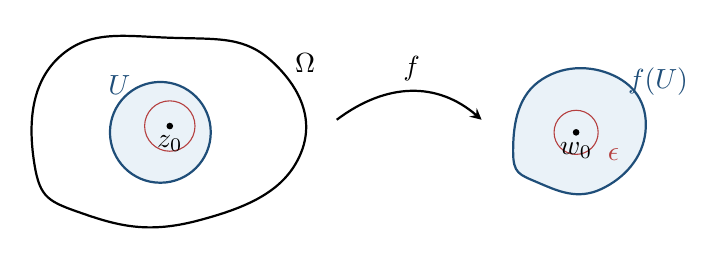
\begin{tikzpicture}[scale=0.8,>=stealth]
 \draw[thick] plot[smooth cycle,tension=0.8] coordinates
 {(-2.6,-0.5) (-2.2,1.2) (-0.4,1.5) (1.2,1.1) (1.6,-0.4) (0,-1.4) (-1.8,-1.3)};
 \node at (1.7,1.1) {$\Omega$};
 \fill[lightblue] (-0.6,0) circle(0.8);
 \draw[courseblue,thick] (-0.6,0) circle(0.8);
 \node[courseblue] at (-1.25,0.75) {$U$};
 \draw[exerciseframe] (-0.45,0.1) circle(0.4);
 \fill (-0.45,0.1) circle(1.5pt) node[below]{$z_0$};
 \draw[->,thick] (2.2,0.2) .. controls (3,0.8) and (3.8,0.8) .. (4.5,0.2)
  node[midway,above]{$f$};
 \begin{scope}[xshift=6cm]
  \fill[lightblue] plot[smooth cycle,tension=0.8] coordinates
   {(-1,-0.3) (-0.6,0.8) (0.6,0.9) (1.1,0) (0.4,-0.9) (-0.6,-0.8)};
  \draw[courseblue,thick] plot[smooth cycle,tension=0.8] coordinates
   {(-1,-0.3) (-0.6,0.8) (0.6,0.9) (1.1,0) (0.4,-0.9) (-0.6,-0.8)};
  \node[courseblue] at (1.3,0.8) {$f(U)$};
  \draw[exerciseframe] (0,0) circle(0.35);
  \fill (0,0) circle(1.5pt) node[below]{$w_0$};
  \node[exerciseframe,right] at (0.35,-0.35) {$\epsilon$};
 \end{scope}
\end{tikzpicture}

{\small Every $w$ within $\epsilon$ of $w_0=f(z_0)$ is attained in the small
disc around $z_0$.}
\end{lecturefigure}

\begin{proof}
The proof follows from Rouch\'e's theorem. Let $w_0\in f(U)$, say
$w_0=f(z_0)$ with $z_0\in U$. We want to show that every $w$ near $w_0$
also lies in the image $f(U)$. Decompose
\[
 f(z)-w=\underbrace{f(z)-w_0}_{F(z)}+\underbrace{w_0-w}_{G(z)}.
\]
Once $w$ is fixed, $G(z)=w_0-w$ is constant in $z$.
The function $F$ has a zero at $z=z_0$. It is not identically zero on
$\Omega$, since $f$ is nonconstant, so by the isolated-zero lemma from Lecture~25 the zero is
isolated: there is $\delta>0$ with $\overline{D(z_0,\delta)}\subseteq U$ and
$F(z)\ne0$ for $0<|z-z_0|\leq\delta$. On the compact circle
$C_\delta=\{|z-z_0|=\delta\}$, $|F|$ has a positive minimum; pick
$\epsilon>0$ with
\[
 |F(z)|=|f(z)-w_0|>\epsilon\qquad\text{for }z\in C_\delta.
\]
Now if $|w-w_0|<\epsilon$, then $|F(z)|>\epsilon>|w-w_0|=|G(z)|$ for
$z\in C_\delta$. By Rouch\'e's theorem, $F+G=f-w$ has as many zeros in
$D(z_0,\delta)$ as $F$, which has at least one (at $z_0$). So $w=f(z)$ for
some $z\in D(z_0,\delta)\subseteq U$. Thus $D(w_0,\epsilon)\subseteq f(U)$,
and $f(U)$ is open.
\end{proof}

\section{The maximum modulus principle}
% Handwritten Lecture 25, Nov. 16, pages 1--2.
\begin{corollary}[Maximum modulus principle]\label{cor:maximum-modulus}
Let $\Omega$ be a connected open set and $f$ holomorphic and nonconstant
on $\Omega$. Then $|f|$ has no local maximum in $\Omega$.
\end{corollary}
\begin{proof}
Suppose $|f|$ has a local maximum at $z_0$. There is an open neighbourhood
$U\subseteq\Omega$ of $z_0$ such that $|f(z)|\leq|f(z_0)|$ for all $z\in U$.
Put $w_0=f(z_0)$. By the open mapping theorem, $f(U)$ is open and contains
$w_0$, so it contains a disc $D(w_0,\epsilon)$ with $\epsilon>0$.
If $w_0\ne0$, the point
\[
 w=w_0+\frac{\epsilon}{2}\frac{w_0}{|w_0|}
\]
lies in this disc and has $|w|=|w_0|+\epsilon/2>|w_0|$.
\begin{lecturefigure}
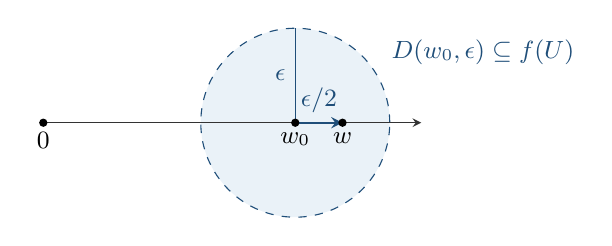
\begin{tikzpicture}[>=stealth,font=\small]
 \coordinate (O) at (0,0);
 \coordinate (W0) at (3.2,0);
 \coordinate (W) at (3.8,0);
 \filldraw[fill=lightblue,draw=courseblue,dashed] (W0) circle (1.2);
 \draw[->,darkgray] (O) -- (4.8,0);
 \draw[courseblue,thick,->] (W0) -- (W) node[midway,above] {$\epsilon/2$};
 \draw[courseblue] (W0) -- ++(0,1.2) node[midway,left] {$\epsilon$};
 \fill (O) circle (1.5pt) node[below] {$0$};
 \fill (W0) circle (1.5pt) node[below] {$w_0$};
 \fill (W) circle (1.5pt) node[below] {$w$};
 \node[courseblue,right] at (4.3,0.9) {$D(w_0,\epsilon)\subseteq f(U)$};
\end{tikzpicture}

{\small Moving from $w_0$ to $w$ along the ray away from the origin
increases the modulus by $\epsilon/2$.}
\end{lecturefigure}
If $w_0=0$, take
$w=\epsilon/2$ instead. In either case, $w=f(z)$ for some $z\in U$, which
contradicts the assumed maximum.
\end{proof}

\begin{remark}[Maximum on the boundary]
Let $\Omega$ be a bounded domain and let $f$ be holomorphic on $\Omega$
and continuous on $\overline{\Omega}$. Then $|f|$ attains its maximum
on the boundary, so
\[
 \max_{z\in\overline{\Omega}} |f(z)|
 = \max_{z\in\partial\Omega} |f(z)|.
\]
Indeed, continuity and compactness give a maximum on $\overline{\Omega}$.
If $f$ is nonconstant, the maximum modulus principle places every point maximizing $|f|$
 on $\partial\Omega$. If $f$ is constant, the maximum is attained
everywhere on $\overline{\Omega}$.
\end{remark}

\section{Analytic isomorphisms}
% Handwritten Lecture 25, pages 2--4. The Rouch\'e and open mapping review
% on page 1 is already included above. The estimates and the choice of a
% punctured disc where f' does not vanish make the multiplicity argument
% on pages 3--4 explicit; openness supplies continuity of the inverse.

\begin{definition}[Analytic isomorphism]
Let $U,V\subseteq\C$ be open. An \emph{analytic isomorphism} from $U$ to $V$
is a bijective holomorphic map $f:U\to V$ whose inverse $g:V\to U$ is also
holomorphic. Equivalently,
\[
 g\circ f=\operatorname{id}_U,\qquad
 f\circ g=\operatorname{id}_V.
\]
We say $U$ and $V$ are \emph{analytically isomorphic} and write $U\cong V$.
The term \emph{biholomorphic} has the same meaning.
\end{definition}

\begin{proposition}\label{prop:analytic-inverse}
Let $U\subseteq\C$ be open and let $f$ be an injective holomorphic function
on $U$. Then $V=f(U)$ is open, and $f:U\to V$ is an analytic isomorphism.
Moreover,
\[
 f'(z)\ne0\quad(z\in U),\qquad
 (f^{-1})'(w)=\frac{1}{f'(f^{-1}(w))}\quad(w\in V).
\]
\end{proposition}
In Lecture~27 we prove this in two steps. First, injectivity forces the derivative to
be nonzero. Then we use a difference quotient to show that the inverse
is holomorphic.

\end{document}
